\documentclass{article}
\usepackage{bera}
\usepackage{float}
\usepackage[margin=1in]{geometry}
\usepackage{graphicx}

\usepackage[colorlinks=true,linkcolor=blue,citecolor=yellow,filecolor=magenta,urlcolor=cyan]{hyperref}
\newcommand{\cymisversion}{0.1-beta}

\begin{document}
\thispagestyle{empty}
\begin{center}
\huge\underline{SDSCSMM v\cymisversion\space User Guide}
\end{center}
\tableofcontents
\clearpage
\pagenumbering{arabic} 
\section{Basic Usage}
\subsection{How to Use}
The mod manager is relatively simple to use if you want to install mods. There are three main stages to mod installation:
\begin{enumerate}
\item Registering mods in the manager
\item Activating registered mods
\item Installing mods to the game archive
\end{enumerate}
We'll go through each of these three steps in the following sections. First, take a moment to familiarise yourself with the annotated image of the user interface in figure \ref{figure:modmanagerui}. We will explore these sections as we go. For now, we'll just cover two sections:
\begin{itemize}
  \item The "Game Executable Location" displays the location of the game on your system. You are prompted to set this the first time the mod manager loads. You can re-set this by clicking the "..." following the text box, if necessary. You should also be prompted to set the location if it is invalid, when the mod manager needs to access it.
  \item The "Message Log" will display time-stamped messages from the mod manager, including error messages if things go wrong. Sometimes this will notify you that a bug has occurred, and sometimes it will tell you that you have tried to do something wrong or that a mod is not set up correctly, but most of the time it should just inform you about what the mod manager is doing when the UI is locked.
\end{itemize}
\begin{figure}[H]\label{figure:modmanagerui}
  \begin{center}
    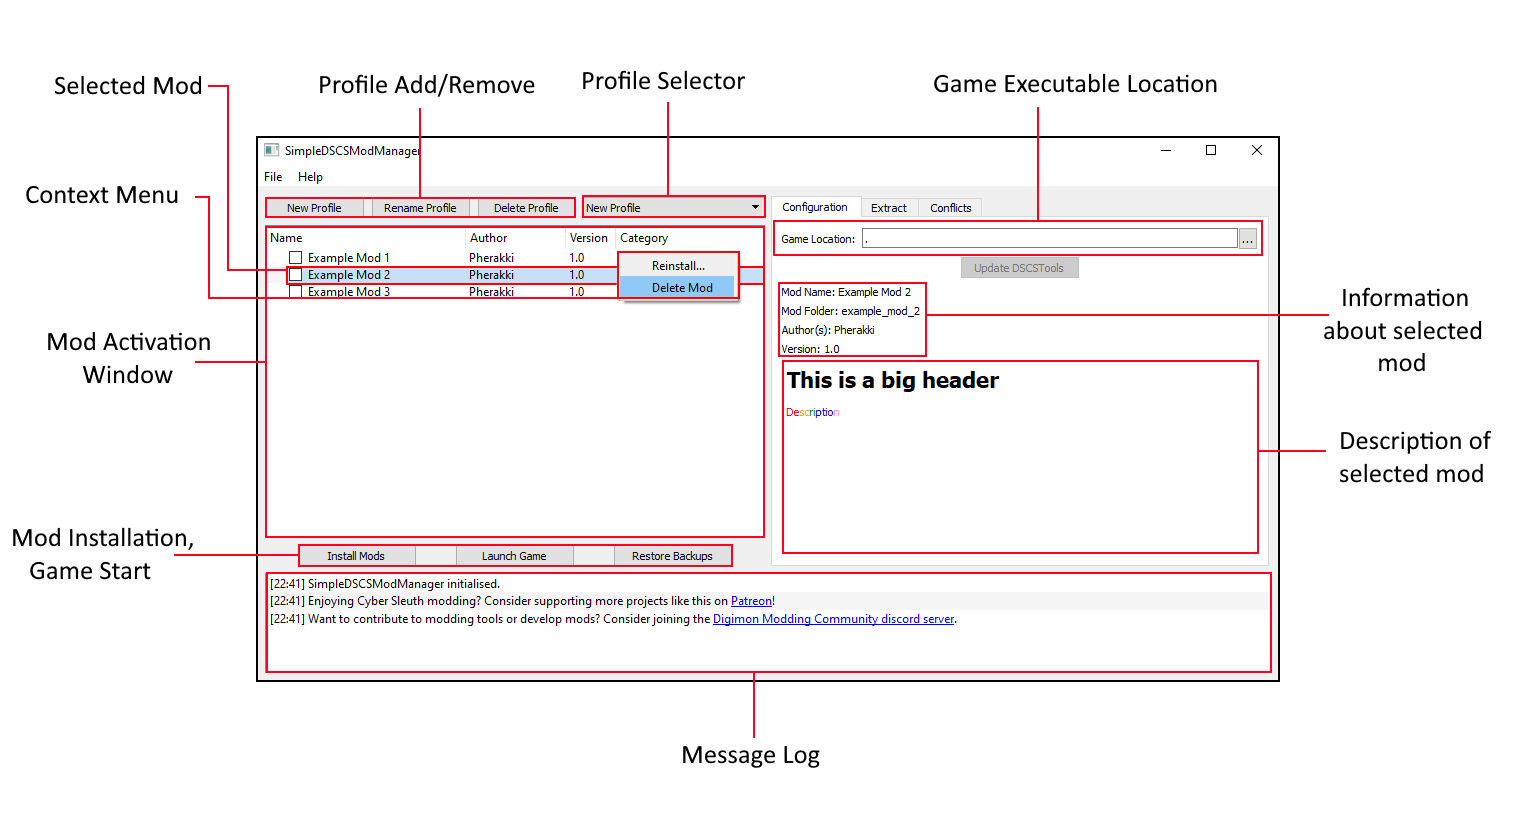
\includegraphics[scale=0.406]{img/modmanager_ui.png}
  \end{center}
  \caption{The mod manager user interface.}
\end{figure}
\newpage

\subsubsection{Registering Mods}
Registering a mod with the manager "installs" the mod to the mod manager. This allows the manager to install the mod into the game files.\\
Registered mods are displayed in the \textbf{Mod Activation Window}.\\\\
There are two ways to register a mod with the manager. The first is to open \textbf{"File > Add Mod..."} in the toolbar, which will open a file dialog. A mod contained in a zip archive an then be selected from this file dialog.\\
The second and arguably simpler way is to drag-and-drop the mod into the \textbf{Mod Activation Window}. Any supported mod format can be installed this way, including an unarchived folder in the correct mod format.
If the mod uses a CYMIS installer, you will be prompted to select what install options you want. It is possible to re-install such a mod with different options \textit{via} the right-click \textbf{context menu}.\\\\
If you ever want to unregister a mod, you can delete the files from the mod manager \textit{via} the right-click \textbf{context menu}.

\subsubsection{Activating Mods with Profiles}
This mod manager makes use of a \textbf{profile} system to allow different combinations of mods to be installed. You can switch between profiles by clicking the \textbf{profile selector}, which will display all the profiles you have created.\\
You can add, rename, and remove profiles by using the buttons to the left of the \textbf{profile selector}. Note that at least one profile must always be present, and the mod manager will prevent you from deleting the final profile.\\
To select which mods are to be installed by the \textbf{profile}, click the checkboxes next to the mod names. If it is checked, it will be installed during the next step.\\
If you click on a mod in the \textbf{Mod Activation Window}, then metadata about that mod will be displayed in the \textbf{"Configuration"} tab on the right-hand side of the manager. This will summarise the name of the mod, the name of the folder it is registered in in the manager files, the version, and category. Below these data, there is also a space to render a mod description in HTML.

\subsubsection{Installing Mods}
This is by far the simplest step for the user, but also the place where things are most likely to go wrong. Now that you have activated some mods, click the "Install Mods" button below the \textbf{Mod Activation Window}. This will begin the process of patching your selected mods together, and installing them into the game files. Depending on the number and size of the mods that are active, this can take several minutes to complete.\\
The adjacent button will launch the game, for convenience.\\
If you ever want to restore the game to a vanilla state, click the "Restore Backups" button, which is located to the right of the "Launch Game" button.
\newpage

\section{Advanced: Writing Mods, Getting Data, and Extensions}
\subsection{Writing a Compatible Mod}
Mods require two things at a minimum:
\begin{itemize}
\item A folder called \textbf{modfiles}
\item A file called \textbf{METADATA.json} containing a JSON dictionary
\end{itemize}
The "modfiles" folder contains the mod data. It should be structured like an unpacked game archive, with the "modfiles" folder in the place of the folder the unpacked game data would be in (i.e. "modfiles" might contain the folders "data/", "message/", "script64/" \textit{etc}).\\
The \textbf{METADATA.json} can contain five main keys:
\begin{itemize}
\item Name
\item Author
\item Version
\item Category
\item Description
\end{itemize}
All of these should be strings (\textit{i.e.} inside quotes), and additionally the "Description" field may be written in HTML.\\
There are two more keys that may also be used:
\begin{itemize}
\item Archives
\item Rules
\end{itemize}
"Archives" is a dictionary that pairs each file contained in "modfiles" to the archive it should be installed into. By default, every file is installed to \textbf{DSDBP}, but if any files should be installed to different archives (e.g. \textbf{DSDBbgm}) then that can be set using this parameter.\\
"Rules" is a dictionary that pairs each file to the rule that should be used to patch that file together with other files of the same name from other mods. The default rule applied to a file depends on its type:
\begin{itemize}
\item MBE tables (csv files inside a folder ending with .mbe) are set to \textbf{mberecord\_overwrite}
\item Script source code (txt files inside script64/) are set to \textbf{squirrel\_overwrite}
\item All other files are set to \textbf{overwrite}
\end{itemize}
The currently available rules are:
\begin{itemize}
\item \textbf{overwrite} --- replaces any file with the same name
\item \textbf{mberecord\_overwrite} --- overwrites any lines in the target csv with the same IDs as the mod csv, creating new lines if no match exists
\item \textbf{mberecord\_join} --- combines non-zero data in the target csv with non-zero data in the mod csv for lines with the same ID
\item \textbf{squirrel\_overwrite} --- overwrites any functions in the target file with those in the mod file if they share a name, and adds any code outside of a function at the start of the file to the start of the target file
\end{itemize}
These rules allow you to just include the \textbf{new} data your mod provides, without needing to also include original game data that is irrelevant.\\\\
If your mod would benefit from some configuration options upon registry, \textit{e.g.} there is an option of which textures to install, then your mod can also be set up to generate a customised set of "modfiles" with a \textbf{CYMIS document}. The details on how to write a CYMIS document are given in the accompanying text "cymis\_specification". The CYMIS document must be saved as \textbf{"INSTALL.json"} alongside the "modfiles" and "METADATA.json". Note that a CYMIS-ready mod \textbf{should not have any files in "modfiles"}, since they will be wiped if the user ever re-installs the CYMIS-ready mod from within the mod manager.\\
Another use case of the CYMIS documents is to generate a large number of similar files from a single source file, which can substantially reduce the distribution size of a mod.

\subsection{Extracting Data}
Game data can be extracted by heading over to the \textbf{"Extract"} tab of the mod manager. The left-hand column of buttons will extract the game archive named on the button, including the unpacking of MBE database files and the decompilation of scripts. Clicking one of these buttons will open a folder selection dialog, where you can select which folder to extract the data to.\\
The right-hand column of buttons requires you to manually select an archive to pack or unpack. In addition, there are options to pack and unpack folders containing MBEs, and compile or decompile folders containing scripts.

\subsection{Plugins}
Several pieces of manager code are implemented as \textbf{plugins}. This allows key functions of the mod manager to be extended by dropping Python source files into the "plugins" directory. This feature is a work-in-progress and will be expanded upon in the future.

\end{document}